\chapter{Enhance the efficacy of Sybil attacks}
\label{sec:atk}
This study focuses on the influence that the dissemination of false network information has during the construction of the topology of the overlay network and how this enhances other network-level attacks.

The performed attack is a Sybil attack, described in section~\ref{sec:sybil}. Sybil nodes are used to increase the connections with honest nodes the attacker has, thus to have greater control on the data flowing between honest nodes.  

In this study, Sybil nodes drop all transactions to and from a chosen victim to perform a denial-of-service. The reader can infer that the same results are applicable for block-withholding attacks.

As previously stated, malicious nodes disseminate bogus network information: they try to advertise as much as possible the addresses of other attackers through \texttt{addr} messages. Consequently, honest nodes are more likely to connect to malicious nodes.

The setting of the attack is during the construction of the overlay topology: at the start the graph is only a tree and many nodes are on fresh bootstrap. Peers try to setup eight outgoing connections, emulating the behaviour of full nodes (Sec.~\ref{sec:peerdisc}). The way the graph forms is influenced by the network data advertised in this phase.

\section{Attack details}\label{sec:atkdetails}
The attack starts during the creation of the overlay topology, when nodes still have to setup most of their connections.

A group of randomly picked nodes is on fresh bootstrap. The rest of the nodes are instead connected. The starting network graph is a tree, the choice comes from the need to have the sparsest graph possible.

In a series of rounds, nodes start to establish outgoing connections with addresses in their peer database. For honest nodes the upper bound on outgoing connections is eight, whereas there is no limitation for malicious nodes, that can therefore start connections with how many nodes they want. Sybil nodes prioritize connections with honest nodes, avoiding connections between each other.

Nodes on fresh bootstrap have to contact some DNS first. DNSs contain the data of a random subset of the nodes that were part of the network at the start. Their addresses will populate the bootstrapping node's peer database, that will then be able to connect to the network and start establishing more connections.

Network information is propagated through \texttt{addr} messages. These are exchanged upon establishing a connection. Bitcoin Core policy is to relay messages that contain at most ten addresses to a subset of neighbours~\cite{btccode}. For this reason, both attackers and honest nodes include in \texttt{addr} messages no more than ten addresses.

In the attack, honest nodes fill \texttt{addr} messages with a random subset of addresses in their peer database. Malicious nodes advertise only attacking nodes' addresses instead (Fig.~\ref{fig:atkadrr}).

Moreover, Sybils do not relay incoming \texttt{addr} messages, thus hampering the propagation of honest nodes addresses. Attackers work under the assumption that they share network knowledge, which means that once an attacker learns a new address, also all other attackers know it.

\begin{figure}[h]
	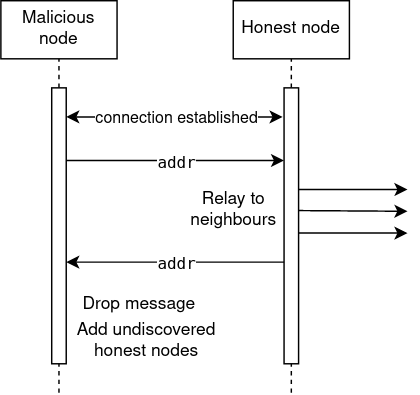
\includegraphics[width=.5\textwidth]{pict/atkaddr.png}
	\centering
	\caption{Peer discovery during the attack}
	\label{fig:atkadrr}
\end{figure}

On top of that, each node self-advertises its address once with an \texttt{addr} message sent to its neighbours. Malicious nodes behave exactly as described before, dropping honest messages.

Once honest nodes cannot establish more connections, and the graph has become dense, the Sybil-based denial-of-service starts: Sybil nodes will drop all the transactions coming from the selected victim.

The Sybil attack has two different settings that lead to different results. In the first one, Sybil nodes are all in network from the start.  In the second, all Sybil nodes are on fresh bootstrap. More can be found in Section~\ref{sec:res}.

\section{Metrics and performance evaluation}\label{sec:metrics}
The tests performed aim to understand how the aforementioned changes in the behaviour of nodes affect the effectiveness of the Sybil-based DoS attacks when adopting different dissemination protocols.

The coverage of a message is defined as the percentage of nodes reached in the network while adopting a certain dissemination protocol.

To evaluate the robustness of fixed probability broadcast and Dandelion ++, the coverage of victims' messages is estimated.

Coverage values for different protocols are carried out through different simulations, while varying the number of attacking nodes and the underlying topology.\par

Other metrics that are used to evaluate the efficacy of the new behaviour of Sybils are the average degree of malicious nodes and the average percentage of malicious neighbours for honest nodes.

These can describe how effectively Sybil nodes have connected to honest nodes, thus influencing the effectiveness of the subsequent Sybils attack.

Furthermore, the average percentage of Sybils in the peer cache is used to assess how well the bogus network information was disseminated.

\section{Software and implementation}\label{sec:softw}
The adopted simulator is LUNES-blockchain, a discrete-time event-based cryptocurrency-system simulator~\cite{lunes-paper}.

It consists of three main modules executed separately: topology creation, blockchain simulation and performance evaluation.

Topology creation is managed with the C library i-graph. Ideally, for each simulation a different set of graphs is generated.

Then the core simulation is run. Nodes mine blocks for the blockchain and exchange transactions with a previously specified dissemination protocol. The Sybil attack is carried out at this time.

At the end of the simulation, some scripts parse the data logged during the simulation and evaluate the robustness of the dissemination protocol.

The changes made to the behaviour of nodes apply only to the first part of the simulation: when nodes are still establishing outgoing connections. Only after this phase, the blockchain simulation is run and the Sybil attack is executed.

It is relevant to point out that the behaviour of nodes emulates as closely as possible that of Bitcoin full nodes.

The simulation proceeds as a series of epochs. In each epoch a different victim is randomly chosen among honest nodes, while the Sybil nodes are still the same from epoch to epoch.

All the tests are a collection of simulations. From a simulation to another the number of Sybil nodes is increased by some proportion of the total number of nodes in the network.

In the second attack scenario, when Sybils are all on fresh bootstrap, the number of total attackers in the network has been increased. Each run adds 100 Sybil nodes and the whole simulation is composed of 300 runs, for a total of 30000 attacking nodes.

On top of that, Sybil nodes join sequentially the network in the same epoch. This information is relevant to understand the results in Section~\ref{sec:external}.